%\documentclass{article}
%\usepackage[spanish]{babel}
%\usepackage{amssymb, amsmath} %Paquetes matemáticos de la American Mathematical Society
%\usepackage{graphicx}
%\usepackage[%
%    a4paper,       % Tamaño de papel
%    left=2.5cm,    % Margen izquierdo
%    right=2.5cm,   % Margen derecho
%   top=3cm,       % Margen superior
%    bottom=3cm,    % Margen inferior
%    footskip=1.5cm % Espacio para el pie de página
%]{geometry}
%\usepackage{fancyhdr}
%\pagestyle{fancy}
%\fancyhf{}
%\lhead[\leftmark]{Síntesis de Redes Activas - Laboratorio 1}
%\rfoot[]{\thepage}
%\begin{document}
 \section{Circuito I: AMPLIFICADOR DIFERENCIAL}

\subsection{Esquemático y datos}

Se realiza el análisis teórico del circuito que se muestra en la siguiente figura: 
  \begin{figure}[h!]
     \centering
	 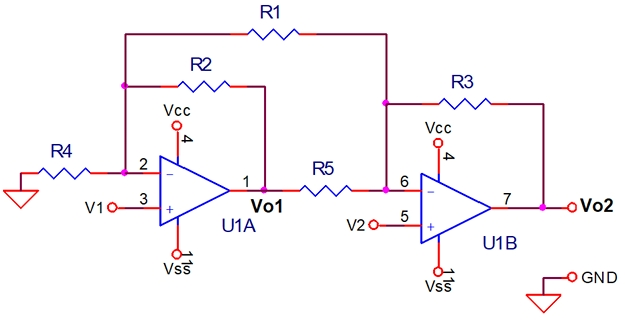
\includegraphics[width=0.6\linewidth]{esquematico1.png}
	 \caption{Esquematico del circuito N° 1}
	 \label{fig:esquematico1}
  \end{figure}
Este circuito consiste en un arreglo de dos amplificadores operacionales cuya función es rechazar la señal común y amplificar la diferencial.

\textbf{Datos:}

\begin{itemize}
  \item Amplificador operacional: LM324
  \item $V_{cc} = 10 \, \text{[V]}$
  \item $V_{ss} = -10 \, \text{[V]}$
  \item $R_1 = R_2 = R_3 = R_4 = R_5 = R$
\end{itemize}

\subsection{Análisis teórico}
Para facilitar el analisis del circuito, se considerará a ambos AO ideales, es decir $V^+=V ^-$ y $A_d=\infty$, se analizarán los AO por separado, y luego se aplicará el teorema de la superposición.

\vspace{1em}

\textbf{Caso $V_2=0$, y $V_1 \neq 0$} 
\vspace{1em}

Pasivada la fuente $V_2$ y analizando las corrientes del nodo de $V^-$ del primer amplificador, resultan las siguientes ecuaciones:

\[-I_1 = I_2 + I_3\]

Esto es: 

\[-\frac{V_1}{R_4} + \frac{V_{o1}-V_1}{R_2} - \frac{V_1}{R_1} = 0\]

\[\frac{V_1}{R_4 + R_2 + R_1}      = \frac{V_{o1}}{R_2}\]

Como $R_1 = R_2 = R_4 = R$

\[V_1\frac{R^2 +R^2 + R^2}{R^3} = \frac{V_{o1}}{R} \]
      
\[V_1 \frac{3R^3}{R^3} = V_{o1} \]

\vspace{1em}

\[3V_1 = V_{o1}\]

Luego, haciendo el mismo análisis para calcular $V_{o2}$ respecto a $V_1$ en el nodo de $V^-$ del segundo amplificador operacional:

\[-I_5 = I_4 + I_3\]

\[\frac{V_{o1}}{R_5} + \frac{V_{o2}}{R_3} + \frac{V_1}{R_1} = 0\]

\[\frac{3V_1}{R_5} + \frac{V_{o2}}{R_3} + \frac{V_1}{R_1} = 0\]

\[\frac{4V_1}{R} + \frac{V_{o2}}{R} = 0\]

\[\Rightarrow \quad -4V_1 = V_{o2} \]

\vspace{1em}

\textbf{Caso $V_1 = 0$ y $V_2 \neq 0$} 

\vspace{1em}

Utilizando la ley de las corrientes en los nodos en la primer etapa:

\[I_{R2} + I_{R1} = 0 \]

\[\frac{V_{01}}{R_2} + \frac{V_2}{R_1} = 0 \]

Como se mencionó antes, todas las resistencias son iguales, por lo que resulta:

\[{V_{01}} = - V_2 \]

Analizando la entrada negativa del segundo AO, las corrientes son definidas:

\[\frac{V_o-V_2}{R_3} - \frac{V_{o1}-V_2}{R_5}+\frac{V_2}{R_1} = 0 \]

\[ V_{o2} - V_2 - V_2 + V_{o1} - V_2 = 0 \]

\[V_{o2} - 4V_2 = 0 \]

\[V_{o2}=4V_2\]

Aplicando la técnica de superposición:

\[V_o = 4V_2  - 4V_1 \]
      
\subsubsection{Análisis de modo diferencial }

Considerando $V_d = V_2 -V_1$ y la tensión de salida calculada anteriormente, resulta

\[ V_o = 4V_d \]
      
\subsubsection{Análisis de modo común}

Sabiendo que $V_c = \frac{V_1 + V_2}{2} $, entonces:

\[ V_2 = \frac{V_{o2}}{4}; \quad  V_1 = -\frac{V_o2}{4} \]

\[ \frac{V_2 +V_1}{2}(4-4) =V_{o2} \]

\[V_{o2} = 0 \]

\subsubsection{RRMC}
Recordando que $RRMC = \frac{A_d}{A_c}$ y, con el análisis realizado de ambos modos, se puede observar que el circuito rechaza por completo el modo común y amplifica el modo diferencial. 
Por lo tanto $RRMC = \infty$

\subsubsection{Impedancias}

Considerando que $Z_i = \frac{V_{in}}{I_{in}} $ y que se tratan de AO ideales, las corrientes de entrada de ambos amplificadores es 0, entonces
\[Z_{i1}=Z_{i2} = \infty \]

\vspace{1em}

\subsection{Simulación y mediciones de laboratorio}

Se realiza la simulación del circuito en el software LTSpice y se arma el circuito de laboratorio respetando los valores de los parámetros simulados.

\vspace{1em}

\subsubsection{Caso $V_2=0$, y $V_1 \neq 0$} 
Las figuras 2 y 3 corresponden a la conexión y la salida para este caso.

\vspace{1em}

  \begin{figure}[h!]
     \centering
     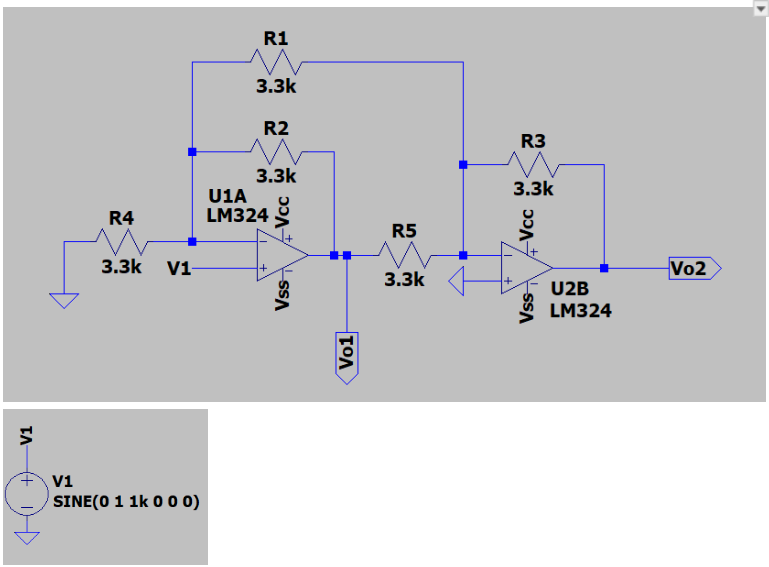
\includegraphics[width=0.5\linewidth]{c1conV2pasivado.png}
     \caption{C 1 - $V_2=0$, y $V_1 \neq 0$}
     \label{fig:enter-label}
 \end{figure}

\vspace{1em}

  \begin{figure}[h!]
     \centering
     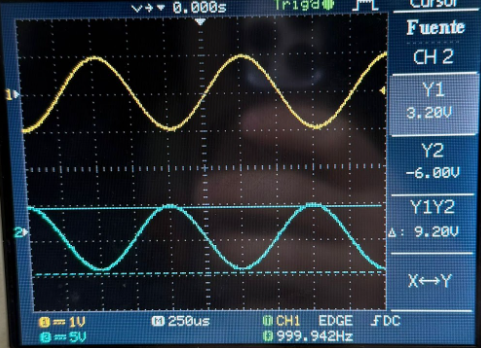
\includegraphics[width=0.4\linewidth]{c1labV2pasivado.png}
     \caption{C 1- medición en osciloscopio para $V_2=0$, y $V_1 \neq 0$}
     \label{fig:enter-label}
 \end{figure}

\vspace{1em}

\subsubsection{Caso $V_1 = 0$ y $V_2 \neq 0$} 
Las figuras 4 y 5 corresponden a la conexión y la salida para este caso.

\vspace{1em}

 \begin{figure}[h!]
     \centering
     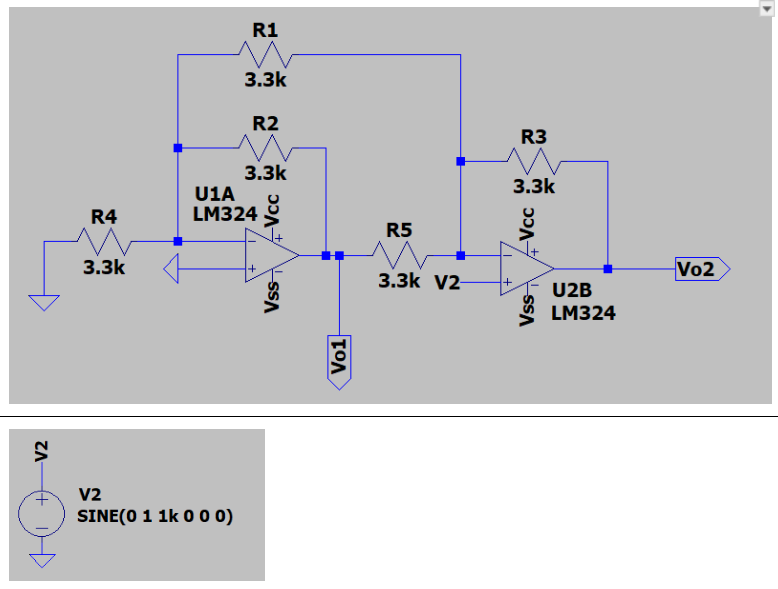
\includegraphics[width=0.5\linewidth]{c1conV1pasivado.png}
     \caption{C 1 -  $V_2 \neq 0$, y $V_1 = 0$}
     \label{fig:enter-label}
 \end{figure}

\vspace{1em}

  \begin{figure}[h!]
     \centering
     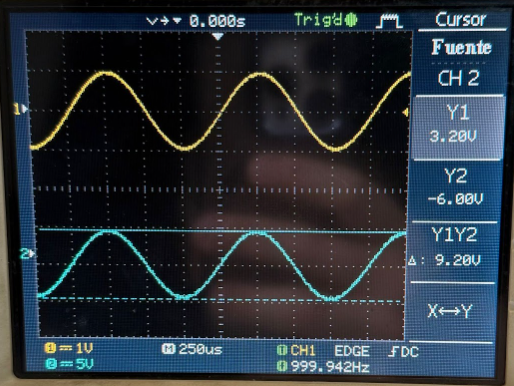
\includegraphics[width=0.4\linewidth]{c1labV1pasivado.png}
     \caption{C 1- medición en osciloscopio para $V_1=0$, y $V_2 \neq 0$}
     \label{fig:enter-label}
 \end{figure}

\vspace{1em}

\subsubsection{Caso $V_{o2} = f(V_d)$} 

 \begin{figure}[h!]
     \centering
     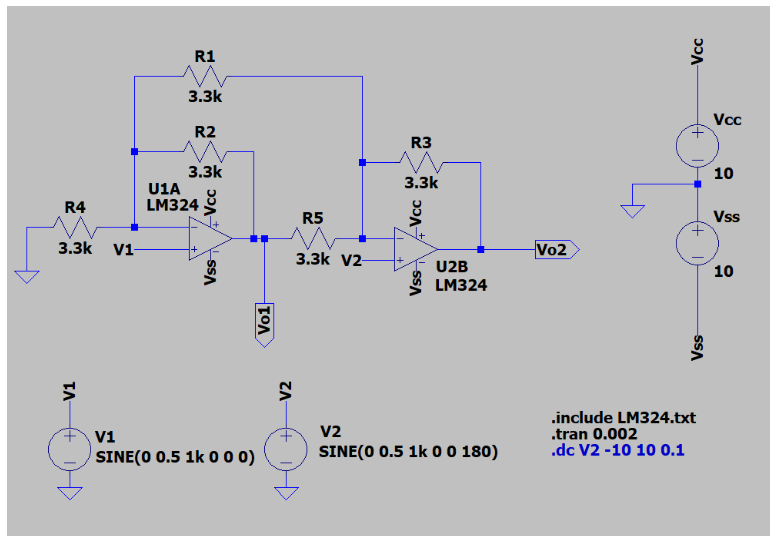
\includegraphics[width=0.5\linewidth]{c1tensionDif.png}    
     \caption{C 1 - tensión en modo diferencial}
     \label{fig:enter-label}
 \end{figure}

\vspace{1em}

\begin{figure}[h!]
    \centering
    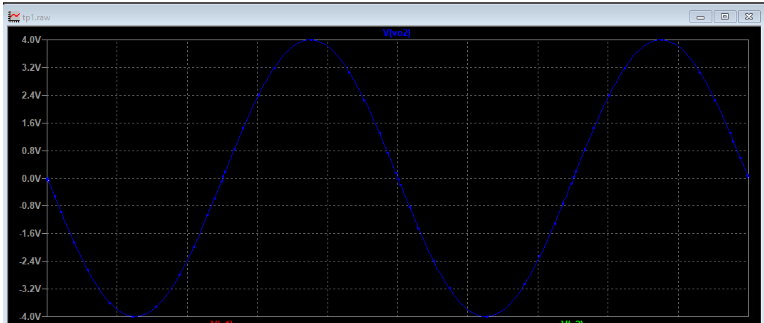
\includegraphics[width=0.6\linewidth]{c1salidaMD.png}    
    \caption{C 1 - Señal de salida para modo diferencial}
    \label{fig:enter-label}
\end{figure}

Se puede ver (figuras 6 y 7) que la tensión de salida simulada en LTSpice es 4 veces la tensión de entrada de modo diferencial como se calculó.
 teóricamente.
Y la tensión medida en el circuito armado es de $V_{o2} = 4,5V_{in}$

\vspace{1em}

\subsubsection{Caso $V_{o2} = f(V_c)$} 

\begin{figure}[h!]
    \centering
    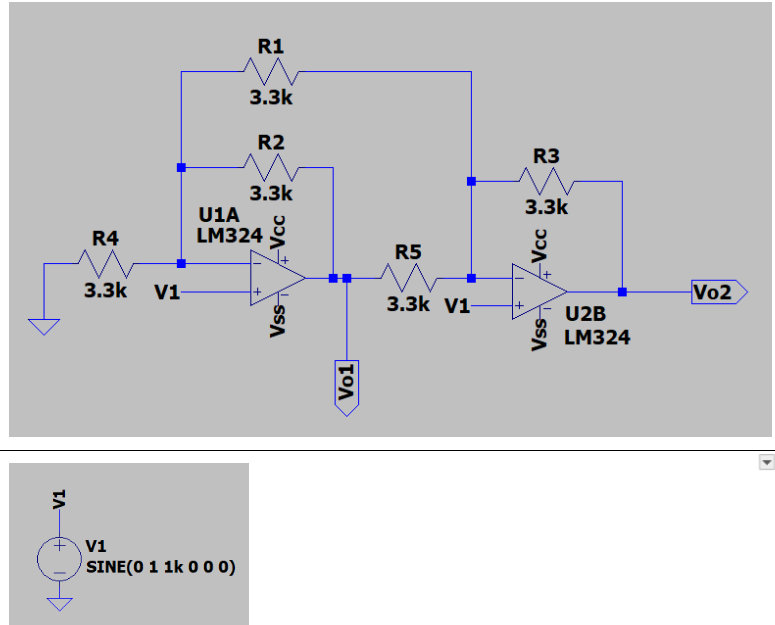
\includegraphics[width=0.5\linewidth]{c1tensionComun.png}    
    \caption{C 1- tensión en modo común}
    \label{fig:enter-label}
\end{figure}

Aplicando una tensión de 1V, se puede notar que la tensión de salida $V_{o2} = 8,2 mV $, es decir no es nula como se dedujo en el análisis teórico, pero sí pequeña.

\begin{figure}[h!]
    \centering
    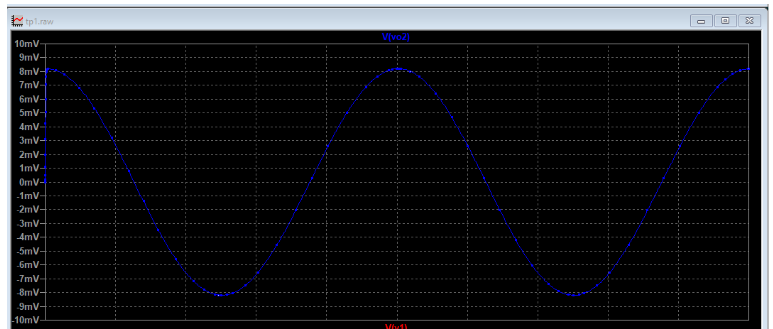
\includegraphics[width=0.6\linewidth]{c1salidaMC.png}    
    \caption{C 1 - Señal de salida para modo común}
    \label{fig:enter-label}
\end{figure}

En el circuito armado se ve que la tensión de salida es $V_{o2} = 16mV $ para 1V en la entrada, y es casi el doble de la simulada.

\begin{figure}[h!]
    \centering
    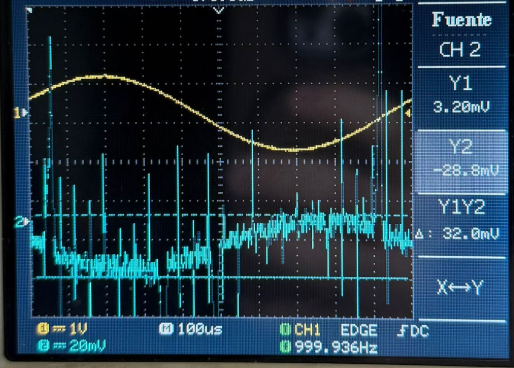
\includegraphics[width=0.4\linewidth]{c1labMC.png}    
    \caption{C1, Señal de salida para modo común medido en el circuito físico}
    \label{fig:enter-label}
\end{figure}

\vspace{1em}

\subsubsection{RRMC}
Las relaciones reales de las gananicas de modo diferencial y de modo común indican que $A_d = 4V_{in}$ y $A_c=8.2mV_{in}$. Luego:

\[ \frac{A_d}{A_c} = \frac{4}{8.2.10^{-03}}\]

\[ \frac{A_d}{A_c} = 487.80\]

Experimentalmente no se obtiene una $RRMC= \infty$ ya que el modo común no es nulo, pero sí es mucho más chico que el diferencial,
 resultando una relación de casi 490 para lo medido en LTSpice y en el laboratorio da:

\[ RRMC= \frac{A_d}{A_c} = \frac{4}{16.10^{-3}} = 218,25 \]


\subsubsection{Impendancias $Z_{i1} y Z_{i2}$}
 Midiendo las corrientes de entrada de ambos AO se pueden calcular los valores de las impedancias de entrada.

\begin{figure}[h!]
    \centering
    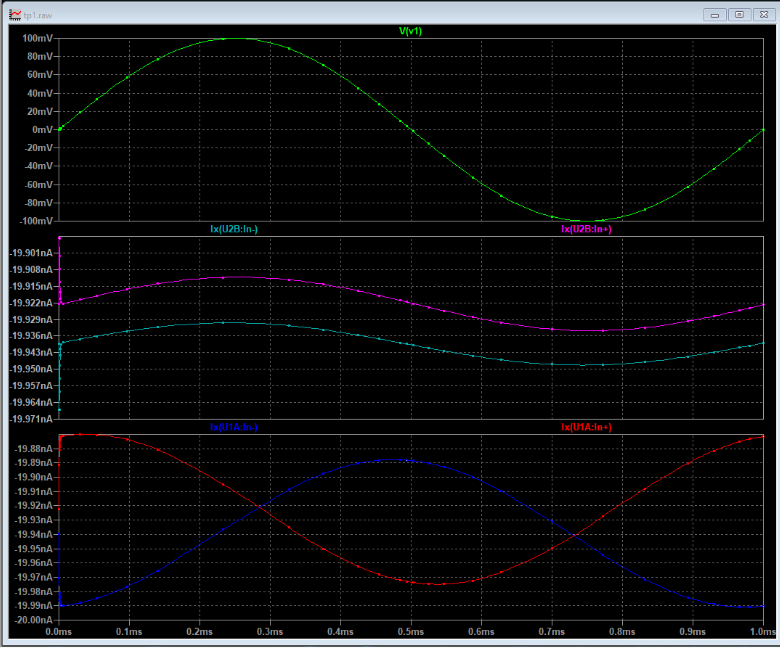
\includegraphics[width=0.7\linewidth]{c1paraImpedancias.png}    
    \caption{Medición de las corrientes de entrada con Vc = 100mV}
    \label{fig:enter-label}
\end{figure}

Se aplicó una tensión de entrada de 100mV y tomando las ecuaciones

\[ Z_{i1} = \frac{V_c}{I_{i1}} \qquad  Z_{i2} = \frac{V_c}{I_{i2}} \]

 Las corrientes medidas, como se muestra en la figura, permiten calcular las impedancias:

\[ Z_{i1} = \frac{100 mV}{19.87 nA} = 5,03 M \Omega \]

\[ Z_{i1} = \frac{100 mV}{19.99 nA} = 5 M \Omega \]

El valor medido difiere de lo planteado teóricamente ($Z_i =\infty$), pero de todas formas, ambas impedancias toman valores muy grandes, en el orden de los $5M\Omega$.

Para la medición de las corrientes en el circuito elaborado físicamente, se presentó la limitación de que los amperímetros disponibles no llegaban a hacer una lectura de valores en nanoAmperes, por lo que no se pudo hacer los cálculos correspondientes. Por lógica se deduce que las impedancias de entrada son muy altas pero no infinitas, ya que se trabaja con AO reales.

%\end{document}